\chapter{Mid fidelity prototype}

\section{Prototype}
The second prototype of the project is the Mid fidelity prototype. The improvement here is the interaction, the interface didn't change much other then some scaling and logo. We took some of the advice from the peer-review from the lo-fi prototype.\\
The prototype is made in balsamiq, a prototype mockup program.\\
Below is a screen-clipping of the welcome screen.
\begin{figure}[H]
\centering
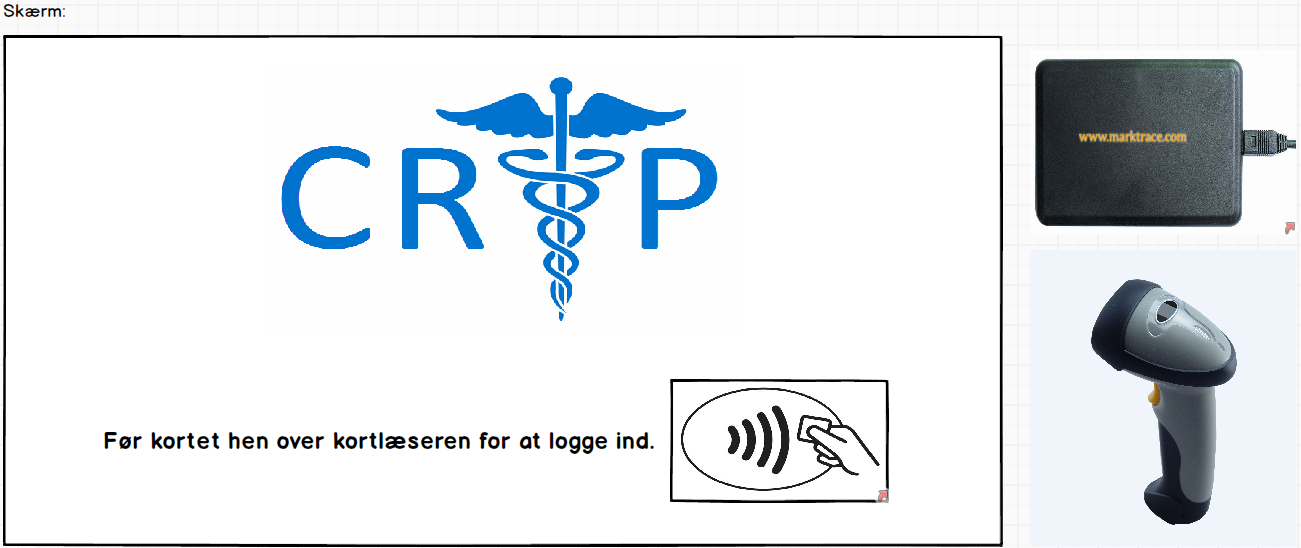
\includegraphics[width=.9\textwidth]{billeder/WelcomeScreen_MidFi}
\caption{Welcome screen in the mid-fi prototype}
\end{figure}
The pictures simulates the RFID scanner which makes it possible to login to the system. The prototype is made on a device with a touchscreen so it is possible to navigate the menus with touch.\\
In balsamiq you can link between different mockups so buttons can be used to navigate through the prototype.\\
So by tapping the RFID scanner the user logs into the system. Below is shown the first page upon login.\\
\begin{figure}[H]
\centering
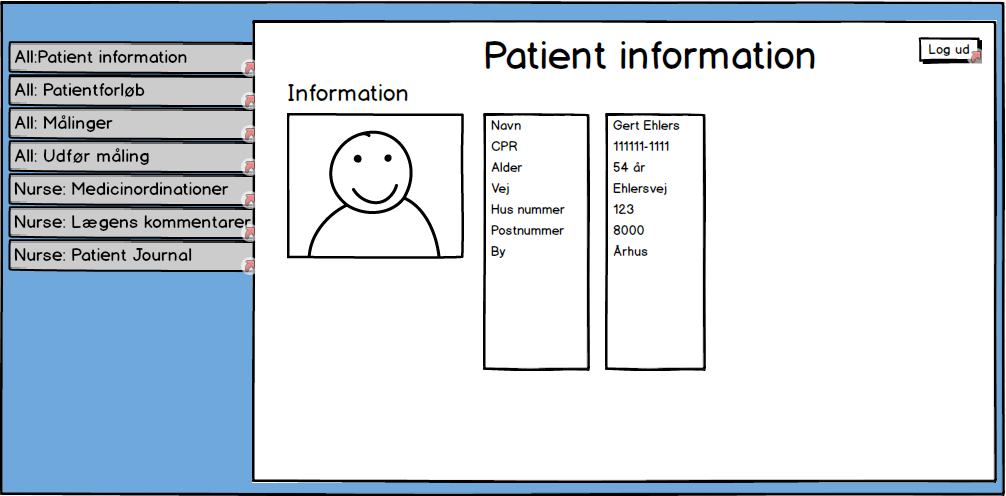
\includegraphics[width=.9\textwidth]{billeder/PatientInformation_MidFi}
\caption{First page, Patient Information, upon login to the CRIP system}
\end{figure}
The mid-fi prototype gives a better feel of the real product then the low-fi.\\
It does this because the navigation have a better feel and the prototype is visually pleasing.\\
The touch feature enables the user to use the prototype as intended which was not possible with the low-fi prototype.\\
In the peer reviews from the low-fi prototype we got some feedback which was applied to the mid-fi.\\
Some of these changes included:\\
\begin{itemize}
\item Bigger buttons
\item More explanatory text
\item Results and important text on top
\end{itemize}

\section{Peer review session outcomes}
respons etc.

\section{Application of prototyping methods, materials and acquired user data}
Hest

\section{Application of evaluation methods, metrics, and statistics}
Math